\subsection{Phoneme discrimination}
\label{sec:abx}

\citet{schatz2013evaluating} propose a framework for evaluating speech features learned in an 
unsupervised setup that does not depend on phonetically labeled data. They propose a set of 
tasks called Minimal-Pair ABX tasks that allow to make linguistically precise comparisons 
between syllable pairs that only differ by one phoneme. They use variants of this task to study 
phoneme discrimination across talkers and phonetic contexts as well as talker discrimination 
across phonemes.

Here we evaluate the COCO~Speech model on the {\it Phoneme across Context} (PaC) task of 
\citet{schatz2013evaluating}. This task consists of presenting a series of equal-length tuples 
$(A, B, X)$ to the model, where $A$ and $B$ differ by one phoneme (either a vowel 
or a consonant), as do $B$ and $X$, but $A$ and $X$ are not minimal pairs.  For example, 
in the tuple ({\it be} /bi/, {\it me} /mi/, {\it my} /\textipa{maI}/),
the task is to identify which of the two syllables /bi/ or /mi/ is closer to /\textipa{maI}/.  The goal is to 
measure context invariance in phoneme discrimination by evaluating how often the model 
recognizes $X$ as the syllable closer to $B$ than to $A$.

\begin{table}
 \centering
 \caption{Accuracy of choosing the correct target in an ABX task using different 
 representations.}
 \label{tab:abx}
 \vspace{.2cm}
 \begin{tabular}{lr}
   \toprule
 { Representation} & {Accuracy} \\
 \midrule
 MFCC &  0.72 \\
 Convolutional & 0.73 \\
 Recurrent 1 &  0.83 \\
 Recurrent 2 &  0.84 \\
 Recurrent 3 &  0.80 \\
 Recurrent 4 &  0.77 \\
 Recurrent 5 &  0.75 \\
 Embeddings  &  0.67 \\
 \bottomrule
 \end{tabular}
 \end{table}


We used a list of all attested consonant-vowel (CV) syllables of American English according to 
the syllabification method described in \citet{Gorman2013}. We excluded the ones which could 
not be unambiguously represented using English spelling for input to the TTS system 
(e.g.\ /\textipa{baU}/). We then compiled a list of all possible $(A, B, X)$ tuples from this list 
where $(A,B)$ and $(B,X)$ are minimal pairs, but $(A,X)$ are not. 
This resulted in 34,288 tuples in total. For each tuple, we measure 
$\mathrm{sign}(\mathrm{dist}(A,X) - \mathrm{dist}(B,X))$, where $\mathrm{dist}(i,j)$ is the 
euclidean distance between the vector 
representations of syllables $i$ and $j$. These representations are either the audio feature 
vectors or the layer activation vectors. A positive value for a tuple means that the model has 
correctly discriminated the phonemes that are shared or different across the syllables.

Table~\ref{tab:abx} shows the discrimination accuracy in this task using various representations. 
The pattern is similar to what we observed in the phoneme identification task: best accuracy is 
achieved using representation vectors from recurrent layers 1 and 2, and it drops as we move 
further up in the model. The accuracy is lowest when final embedding features are used for this task. 




\begin{figure}[t]
  \centering
  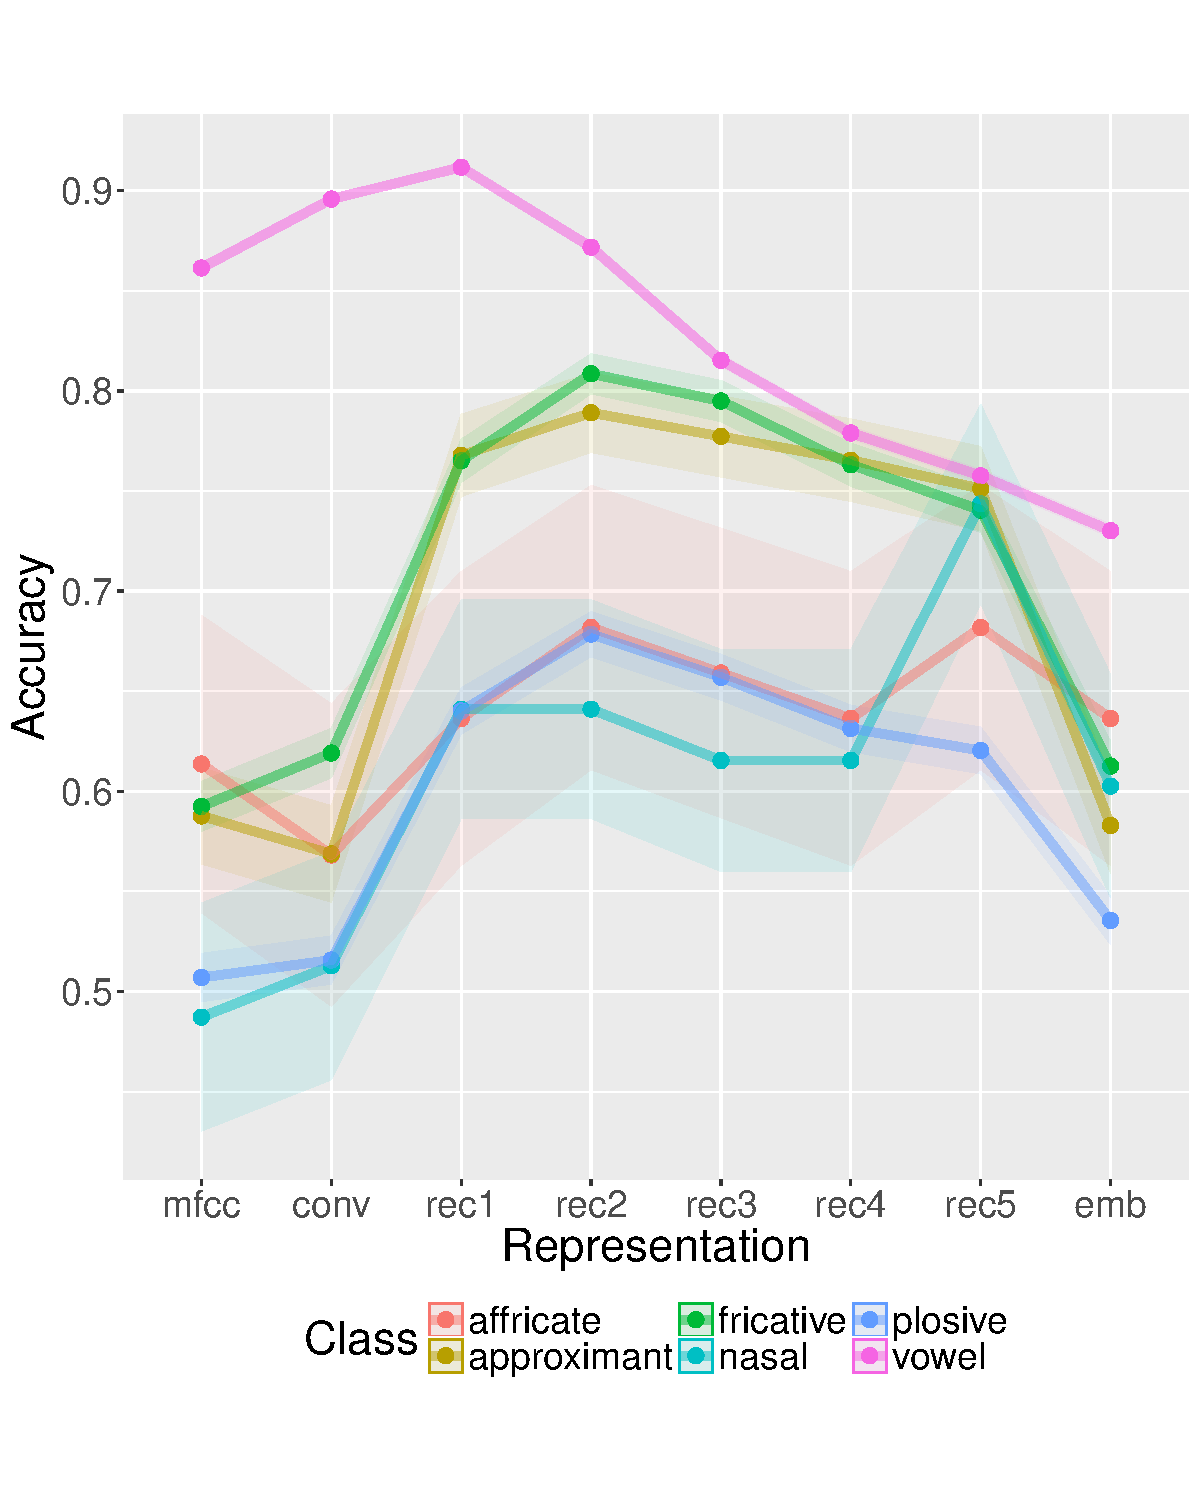
\includegraphics[scale=0.3]{figures/abx_cv_same.pdf}
  \caption{Accuracies for the ABX CV task for the cases where the target
    and the distractor belong to the same phoneme class. Shaded area
    extends $\pm1$ standard error from the mean.}
  \label{fig:abx_cv_same}
\end{figure}

However, the PaC task is most meaningful and challenging where the target and the distractor 
phonemes belong to the same phoneme class. Figure~\ref{fig:abx_cv_same} shows the 
accuracies for this subset of cases, broken down by class.
%
As can be seen, the model can discriminate between phonemes with high accuracy across all 
the layers, and the layer activations are more informative for this task than the MFCC features. 
Again, most phoneme classes seem to be represented more accurately in the lower layers (1--3), and the performance of the model in this task drops as we move towards higher hidden layers. There are also clear differences in the pattern of discriminability for the phoneme classes. The vowels are especially easy to tell apart, but accuracy on vowels drops most acutely in the higher layers. Meanwhile the accuracy on fricatives and approximants starts low, but improves rapidly and peaks around recurrent layer~2. 
The somewhat erratic pattern for nasals and affricates is most likely due to small sample size for these classes, as evident from the wide standard error. 
